\chapter{駐定作用量與尤拉--拉格朗日方程}

\lectureoverview{熟悉的名稱\emph{最小作用量原理}掩蓋了關鍵之處：物理軌跡使作用量取駐值，但不一定使它取極小值。我們將從一般的平衡問題建立這個論述，將它從點推廣到整個函數，藉由離散化路徑推導尤拉--拉格朗日方程，並導出牛頓方程。接著，旋轉座標與極座標將說明，拉格朗日表述不只是改變記號而已。}

\section{取駐值，不一定取極小值}

傳統名稱中不可靠的是\emph{最小}一詞。經典軌跡不一定使作用量取極小值；在所有可能軌跡構成的空間中，它也可能對應極大值或鞍點。正確的原理是作用量\emph{取駐值}：它的一階變化為零。

先從較簡單的平衡問題談起。靜止不動的粒子沒有加速度，因此合力必須為零。若力來自一維勢能，
\begin{equation}
  F(x)=-\frac{dV}{dx},
  \label{eq:force-from-v}
\end{equation}
平衡條件就是
\begin{equation}
  \frac{dV}{dx}=0.
  \label{eq:stationary-v-one}
\end{equation}

\begin{figure}[htbp]
  \centering
  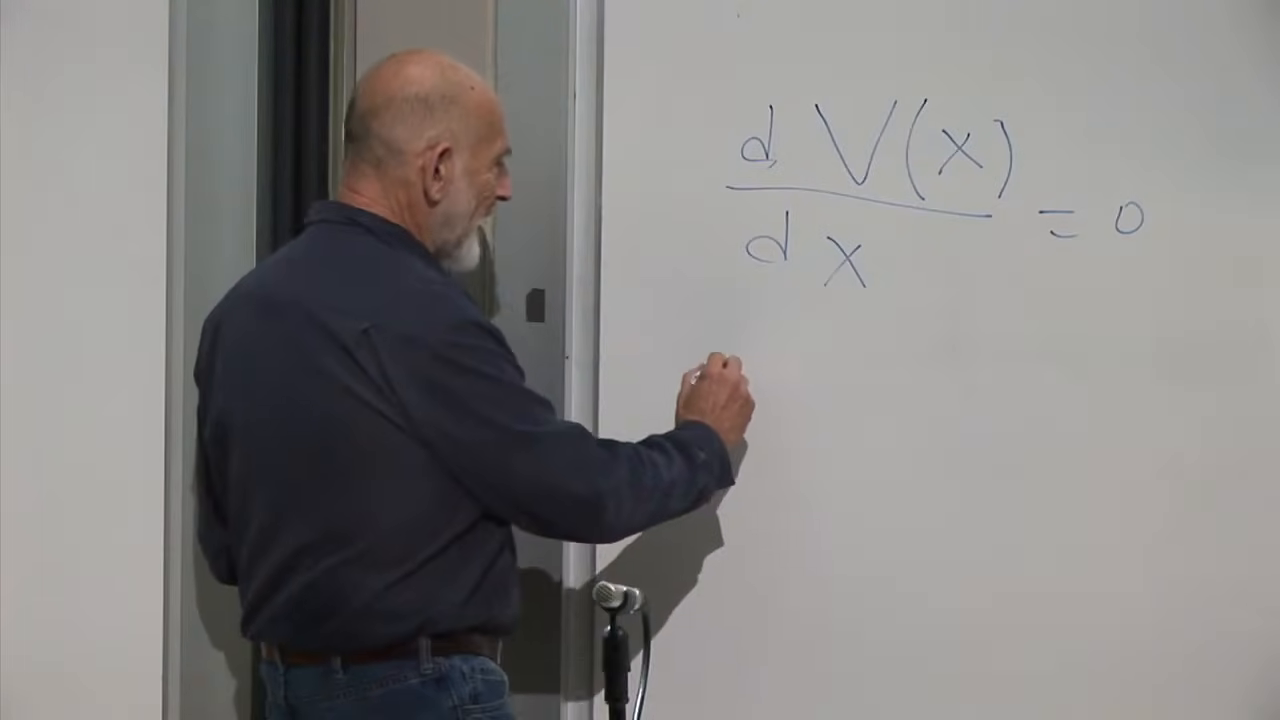
\includegraphics[width=0.74\textwidth]{lecture_03_figure_02.png}
  \caption{一維平衡條件：勢能取駐值處，力為零。}
  \lectureframe{00:02:51}
\end{figure}

現在讓粒子位移一小段\(\delta x\)。在一階近似下，
\begin{equation}
  \delta V
  =V(x+\delta x)-V(x)
  =\frac{dV}{dx}\,\delta x+O(\delta x^2).
  \label{eq:first-variation-one}
\end{equation}
在平衡位置，無論\(\delta x\)的正負為何，線性項都為零：
\begin{equation}
  \delta V=0
  \qquad\hbox{to first order.}
  \label{eq:delta-v-zero-one}
\end{equation}
這不表示有限位移後\(V\)完全不變，而是表示其主要變化從二階或更高階才開始。極小值和極大值都符合這個條件。

\begin{figure}[htbp]
  \centering
  \begin{tikzpicture}[scale=0.95,>=Latex]
    \draw[->] (-0.2,0) -- (3.35,0) node[right] {$x$};
    \draw[->] (0,-0.2) -- (0,2.25) node[above] {$V$};
    \draw[blue!65!black,thick,smooth]
      plot coordinates {(0.2,1.85) (0.75,0.85) (1.55,0.35)
                        (2.35,0.85) (3.0,1.85)};
    \fill[red!65!black] (1.55,0.35) circle (2pt);
    \node at (1.55,-0.34) {minimum};
    \begin{scope}[xshift=4.25cm]
      \draw[->] (-0.2,0) -- (3.35,0) node[right] {$x$};
      \draw[->] (0,-0.2) -- (0,2.25) node[above] {$V$};
      \draw[blue!65!black,thick,smooth]
        plot coordinates {(0.2,0.35) (0.75,1.25) (1.55,1.85)
                          (2.35,1.25) (3.0,0.35)};
      \fill[red!65!black] (1.55,1.85) circle (2pt);
      \node at (1.55,-0.34) {maximum};
    \end{scope}
  \end{tikzpicture}
  \caption{駐定條件決定一階導數，卻不能判定該點是極小值還是極大值。}
  \label{fig:min-max-stationary}
\end{figure}

對多個座標\(q_i\)而言，一階變分為
\begin{equation}
  \delta V
  =\sum_i\frac{\partial V}{\partial q_i}\,\delta q_i.
  \label{eq:first-variation-many}
\end{equation}
若此式必須對每一個彼此獨立的無窮小位移\(\delta q_i\)都為零，則每個係數都必須為零：
\begin{equation}
  \frac{\partial V}{\partial q_i}=0
  \qquad\hbox{for every }i.
  \label{eq:stationary-v-many}
\end{equation}

二維勢能不妨想成起伏的地形，而不是雲霄飛車的軌道。駐定點可能是谷底、山頂，也可能是鞍點。在鞍點附近，沿一個方向移動，勢能一開始會上升；沿另一個方向移動，勢能一開始則會下降。因此，恢復力在一個方向上可能穩定，在另一個方向上卻不穩定，儘管該點的所有一階導數都為零。

\begin{figure}[htbp]
  \centering
  \includegraphics[width=0.76\textwidth]{lecture_03_figure_06.png}
  \caption{鞍點沿所有方向的一階變化都為零，但沿一個軸向的鄰近位移會使勢能上升，沿另一個軸向的位移則會使勢能下降。}
  \lectureframe{00:08:20}
\end{figure}

在多座標構成的空間中，鞍點比單純的極大值或極小值更常見。因此，\emph{駐定}才是更恰當的用語。條件
\begin{equation}
  \delta V=0
  \label{eq:equilibrium-variation}
\end{equation}
概括了平衡狀態，卻不預先判定二階變化的性質。

\section{從點推廣到函數}

力學探討的是完整的運動，而非孤立的平衡點。軌跡是一個函數，例如\(x(t)\)，也可以由一組函數構成，例如\((x(t),y(t),z(t))\)。藉由改變整個函數，使某個量取駐值的數學方法稱為\emph{變分法}。在將變分法應用於運動之前，先看三個較簡單的例子。

\subsection{最短曲線與測地線}

在平面上固定兩點，並以\(y(x)\)表示兩點之間的一條曲線。對一小段曲線而言，
\begin{equation}
  ds=\sqrt{dx^2+dy^2}
  =dx\sqrt{1+\left(\frac{dy}{dx}\right)^2},
  \label{eq:line-element}
\end{equation}
最後一種寫法假設\(dx>0\)。整條曲線的長度是以下泛函：
\begin{equation}
  S[y]=\int_{x_0}^{x_1}
  \sqrt{1+y'(x)^2}\,dx.
  \label{eq:arc-length-functional}
\end{equation}
方括號表示\(S\)的輸入是整個函數。若曲線的小幅變化不改變兩端點，則滿足
\begin{equation}
  \delta S=0
  \label{eq:stationary-length}
\end{equation}
的曲線就是直線。

\begin{figure}[htbp]
  \centering
  \includegraphics[width=0.78\textwidth]{lecture_03_figure_07.png}
  \caption{兩個固定端點之間的一條試探曲線。曲線長度是各無窮小斜邊\(ds\)的總和。}
  \lectureframe{00:13:36}
\end{figure}

同樣的問題也可以在曲面上提出。把繩子在兩根樁之間拉緊，就能直觀呈現受限條件下的最短路徑。這種長度取駐值的曲線稱為\emph{測地線}。在平面上，測地線是直線；在球面或起伏的曲面上則通常不是。

\subsection{費馬原理}

在光速隨位置改變的介質中，光線\(c(x,y)\)不一定沿空間距離最短的路徑前進。光線通過一小段路徑所需的時間，是路段長度除以當地光速，因此
\begin{equation}
  T[y]
  =\int_{x_0}^{x_1}
  \frac{\sqrt{1+y'(x)^2}}{c(x,y)}\,dx.
  \label{eq:fermat-functional}
\end{equation}
費馬原理要求
\begin{equation}
  \delta T=0.
  \label{eq:fermat-stationary}
\end{equation}
當\(c\)為常數時，這就化為最短距離問題。但在折射率不均勻的介質中，最快的路徑必須兼顧路程長短與當地的傳播速度。

\begin{figure}[htbp]
  \centering
  \includegraphics[width=0.80\textwidth]{lecture_03_figure_08.png}
  \caption{光線在局部光速隨位置改變的介質中所需時間的泛函。}
  \lectureframe{00:22:50}
\end{figure}

一則應景的笑話提到當時新近出現的說法：中微子在義大利移動得異常快。物理論述隨即回到可靠的例子：普通光在物質中的速率會依折射率而改變。

\subsection{懸鏈}

兩端固定的鏈條會形成懸鏈線。鏈條的每一小段都貢獻重力位能，因此總位能本身就是沿鏈條積分所得。和前面的例子一樣，端點固定、未知形狀是一個函數，而某個積分必須取駐值。

\begin{figure}[htbp]
  \centering
  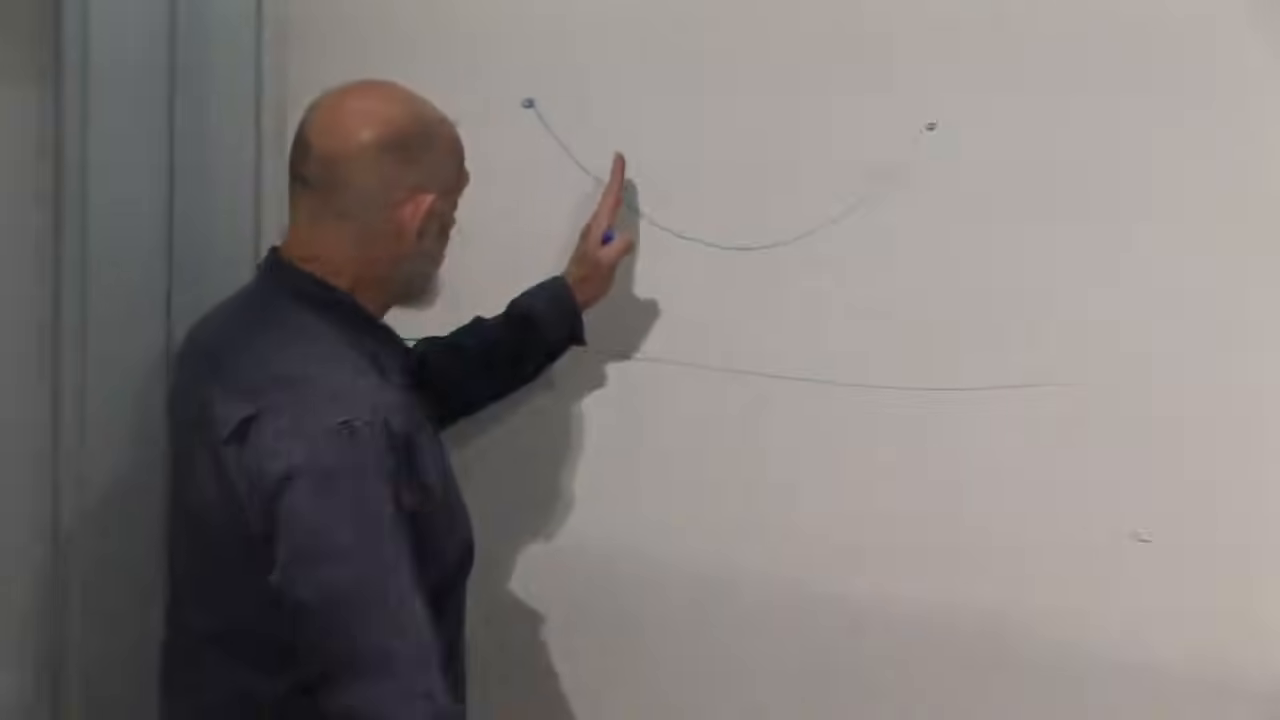
\includegraphics[width=0.76\textwidth]{lecture_03_figure_03.png}
  \caption{懸掛於固定支點之間的鏈條。其駐定形狀由總重力位能決定。}
  \lectureframe{00:30:41}
\end{figure}

這些例子有相同的架構：兩個固定端點、連接端點的函數，以及一個一階變分為零的積分。將這個整體條件化為微分方程，就是求解變分問題。

\section{力學中的邊界值問題}

畫軌跡時，通常把時間畫在水平軸上，因為\(t\)是自變數。不過，物理學中也有一個強烈的慣例：把時間畫成向上延伸。這裡插敘一則實驗：受試者依照與自身書寫系統相關的方向，排列從年輕到年老的人像；習慣由左至右閱讀的人多半由左至右排列，習慣由右至左閱讀的人則反向排列，而習慣縱向閱讀的人則縱向排列。笑話最後說，物理學家就是堅持時間向上流動的人。這裡仍採用慣例中的水平\(t\)軸，因為如此一來，\(x(t)\)自然可視為一張圖。

在初值問題中，\(t_0\)時刻給定的資料是
\begin{equation}
  x(t_0)=x_0,
  \qquad
  \dot x(t_0)=v_0.
  \label{eq:initial-value-data}
\end{equation}
牛頓方程接著決定此後的軌道。變分表述提出的是另一種問題：指定兩個端點事件，
\begin{equation}
  x(t_0)=x_0,
  \qquad
  x(t_1)=x_1,
  \label{eq:boundary-value-data}
\end{equation}
再求出兩事件之間的物理路徑。此時初速度不再是已知條件，而是解的一部分。

\begin{figure}[htbp]
  \centering
  \includegraphics[width=0.76\textwidth]{lecture_03_figure_09.png}
  \caption{一條力學軌跡\(x(t)\)。可以指定一端的位置與斜率，也可以指定兩個端點時刻的位置。}
  \lectureframe{00:27:41}
\end{figure}

要取駐值的量是\emph{作用量}：
\begin{equation}
  A[x]=\int_{t_0}^{t_1}L(x,\dot x,t)\,dt.
  \label{eq:action-one}
\end{equation}
被積函數\(L\)稱為\emph{拉格朗日量}，它可以依賴位置、速度，也可以顯式依賴時間。作用量原理寫作
\begin{equation}
  \delta A=0
  \label{eq:stationary-action}
\end{equation}
並要求路徑變分滿足
\begin{equation}
  \delta x(t_0)=\delta x(t_1)=0.
  \label{eq:fixed-endpoint-variations}
\end{equation}
端點條件至關重要：我們比較的是連接相同兩個事件的鄰近路徑。

\section{尤拉--拉格朗日方程的離散推導}

作用量是以無窮多個路徑上的函數值為輸入的泛函。為了具體計算它的變分，將時間區間切分成長度為\(\epsilon\)的小段，
\begin{equation}
  t_n=t_0+n\epsilon,
  \qquad
  x_n=x(t_n),
  \label{eq:discrete-times}
\end{equation}
並以以下差分近似第\(n\)個區間上的速度：
\begin{equation}
  v_n=\frac{x_{n+1}-x_n}{\epsilon}.
  \label{eq:discrete-velocity}
\end{equation}
於是，積分就成為一般的有限和：
\begin{equation}
  A_\epsilon
  =\sum_{n=0}^{N-1}
  \epsilon L\left(x_n,\frac{x_{n+1}-x_n}{\epsilon}\right).
  \label{eq:discrete-action}
\end{equation}
這裡用\(n\)表示時間切片的標號，讓\(i\)留待後文表示空間座標與粒子。

\begin{figure}[htbp]
  \centering
  \includegraphics[width=0.82\textwidth]{lecture_03_figure_10.png}
  \caption{將軌跡離散成一連串時間切片。改變一個內部點的高度，只會改變相鄰的兩個區段。}
  \lectureframe{00:38:30}
\end{figure}

改變一個內部點\(x_n\)，並保持其他所有\(x_k\)不變。總和中只有兩項依賴\(x_n\)：
\begin{align}
  A_\epsilon\big|_{x_n}
  &=
  \epsilon L\left(x_n,\frac{x_{n+1}-x_n}{\epsilon}\right)
  \notag\\
  &\quad+
  \epsilon L\left(x_{n-1},
                  \frac{x_n-x_{n-1}}{\epsilon}\right).
  \label{eq:two-neighbor-terms}
\end{align}
微分後得到
\begin{align}
  0=\frac{\partial A_\epsilon}{\partial x_n}
  &=
  \epsilon\frac{\partial L_n}{\partial x_n}
  -\frac{\partial L_n}{\partial v_n}
  +\frac{\partial L_{n-1}}{\partial v_{n-1}}.
  \label{eq:discrete-el-variation}
\end{align}
符號相反有簡單的幾何原因：提高\(x_n\)會增大它後方區間的斜率，並減小前方區間的斜率。

\begin{figure}[htbp]
  \centering
  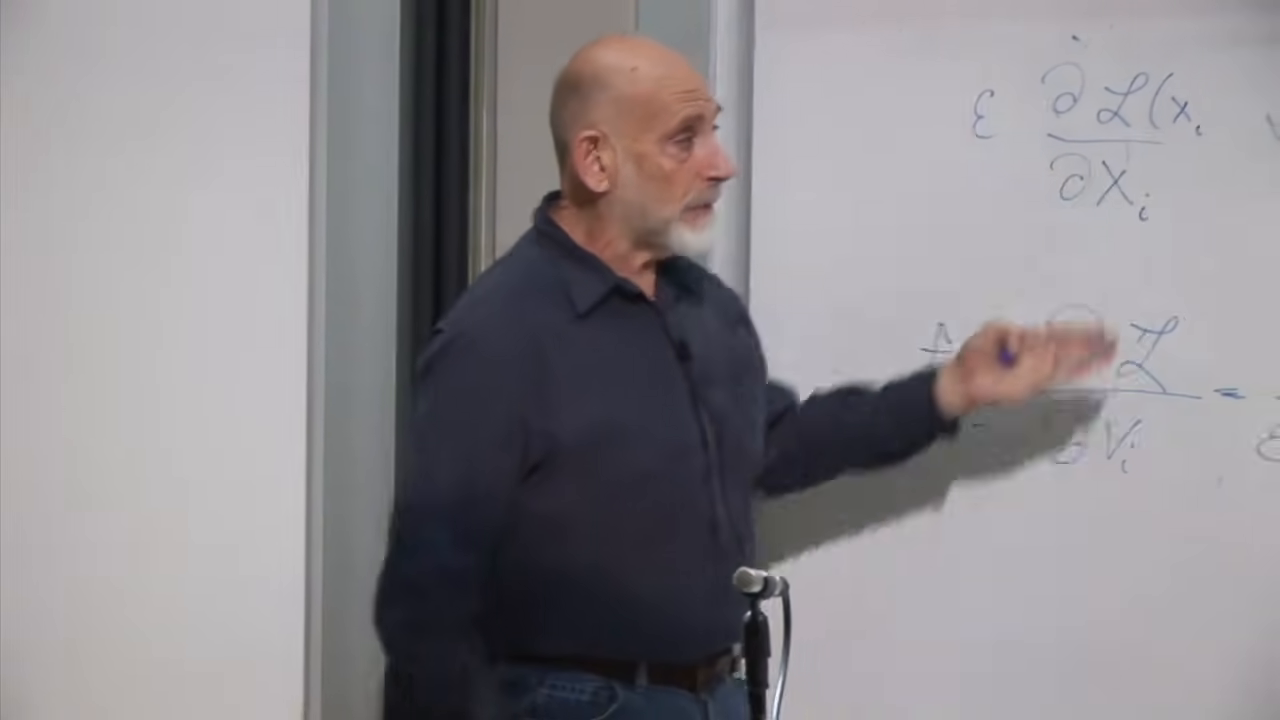
\includegraphics[width=0.74\textwidth]{lecture_03_figure_04.png}
  \caption{離散變分中的直接位置導數，以及兩個相鄰區間對速度導數的貢獻。}
  \lectureframe{00:45:26}
\end{figure}

將式~\eqref{eq:discrete-el-variation}重新整理：
\begin{equation}
  \frac{1}{\epsilon}
  \left(
    \frac{\partial L_n}{\partial v_n}
    -\frac{\partial L_{n-1}}{\partial v_{n-1}}
  \right)
  =
  \frac{\partial L_n}{\partial x_n}.
  \label{eq:discrete-el}
\end{equation}
左側是相鄰兩項的差商。當\(\epsilon\to0\)時，折線趨近光滑路徑，而差商也趨近時間導數：
\begin{equation}
  \boxed{
  \frac{d}{dt}\left(\frac{\partial L}{\partial\dot x}\right)
  =
  \frac{\partial L}{\partial x}}
  .
  \label{eq:euler-lagrange-one}
\end{equation}
這就是尤拉--拉格朗日方程。

\begin{figure}[htbp]
  \centering
  \includegraphics[width=0.78\textwidth]{lecture_03_figure_11.png}
  \caption{在每個內部時間切片都要求駐定後，得到完整的尤拉--拉格朗日方程。}
  \lectureframe{00:49:25}
\end{figure}

給定\(L\)之後，式~\eqref{eq:euler-lagrange-one}就像一部機器：對給定的函數做微分，便能得到路徑所滿足的微分方程。

\begin{classroomqa}
  \audiencequestion{尤拉--拉格朗日方程對任意的\(x\)與\(\dot x\)函數都成立嗎？\lecturetimestamp{00:49:37--00:50:24}}
  \lecturerresponse{是的，但函數必須具備進行所需微分的正則性。
  弧長的例子形式完全相同，只要把自變數\(x\)視為\(t\)，並把未知函數\(y(x)\)視為\(x(t)\)即可。這個例子的尤拉--拉格朗日方程以直線為解。}
\end{classroomqa}

\section{由拉格朗日量導出牛頓方程}

對於位於勢能\(V(x)\)中的直線運動粒子，取
\begin{equation}
  L(x,\dot x)=T-V
  =\frac12m\dot x^2-V(x).
  \label{eq:lagrangian-tv-one}
\end{equation}
負號看來或許奇怪，因為總能量是\(T+V\)。但拉格朗日量並不是能量。判斷它是否正確，要看尤拉--拉格朗日方程能否導出正確的運動。有人提議對正負號模擬投票，但這個提議被婉拒了：答案必須經過檢驗，不能靠投票決定。

首先，
\begin{equation}
  \frac{\partial L}{\partial\dot x}=m\dot x.
  \label{eq:conjugate-momentum-one}
\end{equation}
這就是動量。更一般地，與任意座標\(q\)共軛的動量定義為
\begin{equation}
  p_q=\frac{\partial L}{\partial\dot q}.
  \label{eq:conjugate-momentum-general}
\end{equation}
對式~\eqref{eq:conjugate-momentum-one}取時間導數，得到\(m\ddot x\)；另一方面，
\begin{equation}
  \frac{\partial L}{\partial x}
  =-\frac{dV}{dx}.
  \label{eq:lagrangian-position-derivative}
\end{equation}
因此尤拉--拉格朗日方程為
\begin{equation}
  m\ddot x=-\frac{dV}{dx}=F(x),
  \label{eq:newton-from-action}
\end{equation}
這就是牛頓第二定律。

\begin{figure}[htbp]
  \centering
  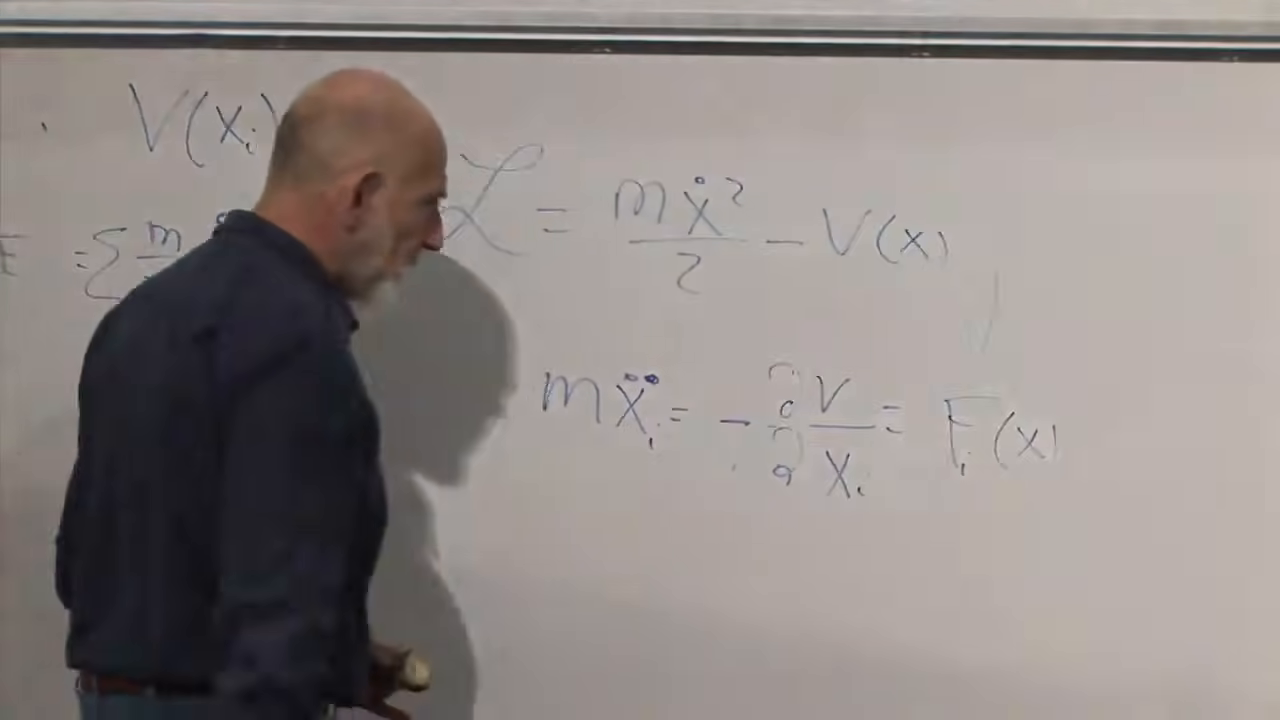
\includegraphics[width=0.80\textwidth]{lecture_03_figure_05.png}
  \caption{同一塊黑板上列出動能、位能、\(L=T-V\)，以及導出的牛頓方程分量形式。}
  \lectureframe{00:57:52}
\end{figure}

對多個座標\(q_i\)而言，
\begin{equation}
  L(\mathbf q,\dot{\mathbf q})
  =\sum_i\frac12m_i\dot q_i^{\,2}-V(q_1,q_2,\ldots),
  \label{eq:lagrangian-tv-many}
\end{equation}
每個座標都對應一個方程：
\begin{equation}
  \frac{d}{dt}\left(\frac{\partial L}{\partial\dot q_i}\right)
  =\frac{\partial L}{\partial q_i}
  \quad\Longrightarrow\quad
  m_i\ddot q_i=-\frac{\partial V}{\partial q_i}=F_i.
  \label{eq:euler-lagrange-many}
\end{equation}
軌跡仍是一條曲線，只是現在位於高維位形空間中。

\begin{classroomqa}
  \audiencequestion{我們是否只是從牛頓定律倒推，刻意構造出一個能重現結果的泛函？\lecturetimestamp{00:58:07--01:00:04}}
  \lecturerresponse{這不是最有成效的觀點。拉格朗日量是物理系統的精簡描述：一個包含所有座標與速度的函數，就能統整系統的所有運動方程。提出新理論時，物理學家通常先提出作用量，再由此推導方程，而不是逐一猜測每個方程。}
\end{classroomqa}

這種統整方式是一項優點，座標自由度則是另一項。直線最短，不會因為用笛卡兒座標、極座標或曲線座標描述平面而改變。同樣地，作用量取駐值的條件與座標系無關，儘管\(L\)的表達式和由此得到的分量方程會隨座標選擇而改變。

\section{從旋轉木馬上看自由粒子}

令\((x,y)\)為慣性笛卡兒座標，\((X,Y)\)為以角速度\(\omega\)均勻旋轉的座標。依照此處採用的方向約定，
\begin{align}
  x&=X\cos\omega t+Y\sin\omega t,
  \notag\\
  y&=-X\sin\omega t+Y\cos\omega t.
  \label{eq:rotating-coordinate-map}
\end{align}
兩座標系的夾角為\(\omega t\)。

\begin{figure}[htbp]
  \centering
  \includegraphics[width=0.76\textwidth]{lecture_03_figure_12.png}
  \caption{慣性笛卡兒座標軸與均勻旋轉的笛卡兒座標軸。同一個點在旋轉座標系中有隨時間變化的座標。}
  \lectureframe{01:06:05}
\end{figure}

自由粒子在慣性系中的拉格朗日量為
\begin{equation}
  L_{\mathrm{in}}
  =\frac{m}{2}\left(\dot x^2+\dot y^2\right).
  \label{eq:free-inertial-lagrangian}
\end{equation}
對式~\eqref{eq:rotating-coordinate-map}微分，並利用
\(\sin^2\omega t+\cos^2\omega t=1\)。三角函數項合併後可得
\begin{align}
  \dot x^2+\dot y^2
  &=
  \dot X^2+\dot Y^2\\
  &\quad+\omega^2(X^2+Y^2)\\
  &\quad+2\omega(Y\dot X-X\dot Y).
  \label{eq:rotating-speed}
\end{align}
因此
\begin{align}
  L_{\mathrm{rot}}
  &=
  \frac{m}{2}(\dot X^2+\dot Y^2)\\
  &\quad+\frac{m\omega^2}{2}(X^2+Y^2)\\
  &\quad+m\omega(Y\dot X-X\dot Y).
  \label{eq:rotating-lagrangian}
\end{align}

\begin{figure}[htbp]
  \centering
  \includegraphics[width=0.84\textwidth]{lecture_03_figure_13.png}
  \caption{變換後的自由粒子拉格朗日量：一般動能、一個二次離心項，以及一個對速度呈線性的項。}
  \lectureframe{01:12:16}
\end{figure}

二次座標項的形式為\(-V_{\mathrm{fict}}\)，其中
\begin{equation}
  V_{\mathrm{fict}}
  =-\frac{m\omega^2}{2}(X^2+Y^2).
  \label{eq:centrifugal-potential}
\end{equation}
此項隨著距離旋轉軸愈遠而減小，因此產生離心力
\(m\omega^2(X,Y)\)。

式~\eqref{eq:rotating-lagrangian}的最後一項對座標與速度都是線性的。套用尤拉--拉格朗日方程可得
\begin{align}
  m\ddot X&=m\omega^2X-2m\omega\dot Y,
  \notag\\
  m\ddot Y&=m\omega^2Y+2m\omega\dot X.
  \label{eq:rotating-equations}
\end{align}
與\(\omega^2\)成正比的項是離心項，與速度成正比的項則是科里奧利項。在旋轉平面內，向量形式為
\begin{equation}
  \mathbf F_{\mathrm{C}}
  =-2m\,\boldsymbol\omega\times\mathbf v_{\mathrm{rot}},
  \label{eq:coriolis-vector}
\end{equation}
若採用相反的方向約定，符號也會相應改變。

\begin{figure}[htbp]
  \centering
  \includegraphics[width=0.84\textwidth]{lecture_03_figure_14.png}
  \caption{旋轉座標系中的方程：與座標成正比的項給出離心加速度，與交叉速度成正比的項則給出科里奧利加速度。}
  \lectureframe{01:20:20}
\end{figure}

重點不在於代數運算消失了，而在於對一個純量函數做一次座標變換，就能同時導出兩個耦合方程與兩種慣性力。

\begin{classroomqa}
  \audiencequestion{這個方法也適用於任意曲線座標嗎？\lecturetimestamp{01:22:01--01:22:17}}
  \lecturerresponse{適用。新座標可以是曲線座標，也可以像旋轉座標一樣顯式依賴時間。只要用新變數改寫作用量，再套用相同的尤拉--拉格朗日法則即可。}
\end{classroomqa}

\section{極座標與循環座標}

在一般極座標中，
\begin{equation}
  x=r\cos\theta,
  \qquad
  y=r\sin\theta.
  \label{eq:polar-map}
\end{equation}
\(r\)和\(\theta\)都可以隨時間變化。對座標取時間導數，再將平方項相加，可得
\begin{equation}
  \dot x^2+\dot y^2
  =\dot r^2+r^2\dot\theta^2.
  \label{eq:polar-speed}
\end{equation}
若中心勢能為\(V(r)\)，則
\begin{equation}
  L
  =\frac{m}{2}\left(\dot r^2+r^2\dot\theta^2\right)-V(r).
  \label{eq:polar-lagrangian}
\end{equation}

\begin{figure}[htbp]
  \centering
  \includegraphics[width=0.80\textwidth]{lecture_03_figure_15.png}
  \caption{極座標幾何，以及動能在徑向運動與角向運動間的分解。}
  \lectureframe{01:23:30}
\end{figure}

徑向方程為
\begin{equation}
  m\ddot r
  =mr\dot\theta^2-\frac{dV}{dr}.
  \label{eq:radial-equation}
\end{equation}
第一項是由粒子自身的角向運動所造成的向外離心效應。

對角座標而言，
\begin{equation}
  \frac{d}{dt}\left(\frac{\partial L}{\partial\dot\theta}\right)
  =\frac{\partial L}{\partial\theta}=0,
  \label{eq:theta-el}
\end{equation}
因為中心勢能沒有顯式的\(\theta\)依賴性。因此
\begin{equation}
  \frac{d}{dt}\left(mr^2\dot\theta\right)=0,
  \qquad
  mr^2\dot\theta=\ell,
  \label{eq:angular-momentum}
\end{equation}
其中\(\ell\)是守恆的角動量。

\begin{figure}[htbp]
  \centering
  \includegraphics[width=0.82\textwidth]{lecture_03_figure_16.png}
  \caption{角座標的尤拉--拉格朗日方程右側為零，因此顯示出\(mr^2\dot\theta\)守恆。}
  \lectureframe{01:29:25}
\end{figure}

角向方程給出
\begin{equation}
  \dot\theta=\frac{\ell}{mr^2}.
  \label{eq:theta-dot-angular-momentum}
\end{equation}
將此結果代入式~\eqref{eq:radial-equation}，便得到只含\(r\)的一個方程：
\begin{equation}
  m\ddot r
  =\frac{\ell^2}{mr^3}-\frac{dV}{dr}.
  \label{eq:effective-radial-equation}
\end{equation}

不出現在\(L\)中的座標，傳統上稱為\emph{循環}座標，即使它不是角度也一樣。若\(q\)是循環座標，則
\begin{equation}
  \frac{\partial L}{\partial q}=0
  \quad\Longrightarrow\quad
  \frac{d}{dt}\left(\frac{\partial L}{\partial\dot q}\right)=0.
  \label{eq:cyclic-conservation}
\end{equation}
其共軛動量便是守恆量。這初步揭示了對稱性與守恆定律之間的一般關係。

\section{關於意義、能量與適用範圍的問題}

接下來的問題將點出這套形式體系更深層的內涵。

\begin{classroomqa}
  \audiencequestion{除了發現拉格朗日量能導出正確的經典方程之外，還有其他獨立的理由可以得到拉格朗日量嗎？\lecturetimestamp{01:33:25--01:35:07}}
  \lecturerresponse{從歷史上看，經典力學在一個多世紀的發展中，已證明粒子、波與電磁場都能寫成這種形式。在經典層次上，這些累積的成功，是關於自然定律如何組織起來的經驗事實。更深層的解釋來自量子力學，這裡暫且不談。}
\end{classroomqa}

\begin{classroomqa}
  \audiencequestion{旋轉座標系中的拉格朗日量裡，對速度呈線性的項能否視為一般的動能或位能？\lecturetimestamp{01:35:08--01:36:23}}
  \lecturerresponse{不能。與時間平移對稱性相關的守恆量，是由哈密頓量的構造方式導出的，不能把\(L\)中的每一項都直接解讀為動能或位能。對式~\eqref{eq:rotating-lagrangian}而言，對速度呈線性的項在\(\sum_a\dot q_a\,\partial L/\partial\dot q_a-L\)中會相消。哈密頓形式將有系統地整理這個問題。}
\end{classroomqa}

確實，由於\(L_{\mathrm{rot}}\)沒有顯式的時間依賴性，
\begin{equation}
  \begin{aligned}
    H_{\mathrm{rot}}
    &=\dot X\frac{\partial L}{\partial\dot X}
     +\dot Y\frac{\partial L}{\partial\dot Y}-L\\
    &=\frac{m}{2}(\dot X^2+\dot Y^2)
     -\frac{m\omega^2}{2}(X^2+Y^2)
  \end{aligned}
  \label{eq:rotating-hamiltonian-preview}
\end{equation}
是守恆量。它是旋轉座標系中的雅可比積分，數值上並不等同於慣性觀察者所賦予的能量。依賴時間的座標變換不一定保留能量的數值形式。

\begin{classroomqa}
  \audiencequestion{如果曲線軌跡是由重力造成的呢？\lecturetimestamp{01:36:30--01:37:10}}
  \lecturerresponse{對於牛頓重力，只要在中心力拉格朗日量中取\(V(r)=-GMm/r\)即可。彎曲時空屬於廣義相對論，這裡不予採用。}
\end{classroomqa}

\begin{classroomqa}
  \audiencequestion{離心位能及其能量只是虛構的嗎？\lecturetimestamp{01:37:13--01:40:14}}
  \lecturerresponse{旋轉平台上的觀察者可以測量有效力，也能一致地使用旋轉座標系中的守恆量。\emph{虛構}表示這些項源自非慣性座標系的描述，並不表示它們造成的可觀測效應是假的。一般而言，能量在依賴時間的座標變換下並非不變。}
\end{classroomqa}

\begin{classroomqa}
  \audiencequestion{與速度相關的科里奧利力指向哪個方向？\lecturetimestamp{01:40:22--01:42:36}}
  \lecturerresponse{它垂直於旋轉座標系中的速度，大小與速率和座標系的角速度成正比。在平面內，兩個分量會分別交換\(\dot X\)與\(\dot Y\)，並帶有相反的符號，如式~\eqref{eq:rotating-equations}所示。}
\end{classroomqa}

\begin{figure}[htbp]
  \centering
  \includegraphics[width=0.76\textwidth]{lecture_03_figure_17.png}
  \caption{交叉速度分量的形式：科里奧利力垂直於旋轉座標系中的速度。}
  \lectureframe{01:41:40}
\end{figure}

\begin{classroomqa}
  \audiencequestion{起始拉格朗日量一定要在慣性系中寫出嗎？\lecturetimestamp{01:42:37--01:44:00}}
  \lecturerresponse{對一般的自由粒子而言，牛頓的慣性系定律提供了簡單的起始形式\(m(\dot x^2+\dot y^2)/2\)。知道這條物理定律後，就可以將作用量轉換到其他任何座標系。不應另外假設旋轉座標系中也有相同的簡單動能公式。}
\end{classroomqa}

磁場中的帶電粒子也會出現同類的速度線性項：
\begin{equation}
  L_{\mathrm{em}}
  =\frac12m\mathbf v^2
   +q\mathbf A(\mathbf r,t)\cdot\mathbf v
   -q\phi(\mathbf r,t).
  \label{eq:electromagnetic-lagrangian}
\end{equation}
若均勻磁場垂直於平面，採用對稱規範\(\mathbf A=\tfrac12\mathbf B\times\mathbf r\)便會產生一個與\(X\dot Y-Y\dot X\)成正比的項，其代數形式與科里奧利項相同。

\begin{figure}[htbp]
  \centering
  \includegraphics[width=0.82\textwidth]{lecture_03_figure_18.png}
  \caption{旋轉座標系中的速度線性項，讓我們得以將它與均勻磁場中的帶電粒子作比較。}
  \lectureframe{01:44:40}
\end{figure}

\begin{classroomqa}
  \audiencequestion{除了光滑性之外，作為拉格朗日量的函數還必須符合哪些條件？\lecturetimestamp{01:44:46--01:45:06}}
  \lecturerresponse{有，但相關限制需要更多尚未介紹的數學架構，因此留待後續討論。現階段的核心要點是：提出一個拉格朗日量，就能由它導出方程與守恆定律。}
\end{classroomqa}

旋轉系方程也允許圓周運動：在慣性系中靜止的點，從旋轉木馬上看會繞著旋轉原點轉動。磁場的類比則說明了帶電粒子為何能作迴旋運動。

\begin{classroomqa}
  \audiencequestion{帶電粒子會一直沿著那個圓運動，還是會因輻射而使軌道塌縮？\lecturetimestamp{01:46:11--01:47:21}}
  \lecturerresponse{目前討論的粒子方程沒有納入輻射。若將粒子與電磁場的耦合以及輻射反作用一併納入，加速的經典電荷便會輻射。因此，輻射是額外的物理效應，並不與簡化方程中的軌道相矛盾。}
\end{classroomqa}

\begin{classroomqa}
  \audiencequestion{颶風與這個討論有什麼關係？
  \lecturetimestamp{01:47:30--01:47:50}}
  \lecturerresponse{颶風的大尺度大氣運動發生在旋轉的地球上，因此科里奧利效應很重要。完整的推導屬於氣象學範疇，這裡不會展開。}
\end{classroomqa}

\begin{classroomqa}
  \audiencequestion{作用量架構預期能涵蓋每一條物理定律嗎？若真有例外，又代表什麼？\lecturetimestamp{01:47:57--01:49:01}}
  \lecturerresponse{在此處討論範圍內，所有已知的封閉基礎理論都能用作用量來組織，包括牛頓粒子、麥克斯威場、廣義相對論與標準模型。黏滯阻力等表面上的反例，是因為省略了環境自由度才出現。若把流體或微觀熱浴也納入系統，基礎描述仍符合這套架構。因此，若發現真正基礎的例外，將會是重大發現。}
\end{classroomqa}